
\begin{multicols*}{2}

\section{Fighter}

\lettrine[lines=3, lhang=0.15, loversize=0.25, findent=.5em]{F}{ighters} rely on stout hearts, brute strength, and melee weapons to subdue their enemies and protect their allies. They generally disdain long-range warfare, preferring instead to charge into the fray swinging their weapon of choice. 

\subsection*{Action Surge}


Starting at 1st level, you can push yourself beyond your normal limits for a moment.
Once per turn, you can use one point of stamina to make on additional attack.



\subsection*{Maneuvers}

At 3rd level, you learn maneuvers that are fueled by your stamina dice.
You learn four maneuvers of your choice. You learn two additional maneuvers of your choice at 7th and 10th level. Note that some maneuvers require you to be holding certain weapons or carrying a shield. Refer to the  fighter's maneuvers table for descriptions.

\textbf{Saving Throws.} Some of your maneuvers require your target to make a saving throw to resist the maneuver's effects. The saving throw DC is calculated as follows:

\textbf{Maneuver save DC} = 8 + your proficiency bonus + your Strength or Dexterity modifier (your choice)


\subsection*{War Shout}

By 7th level, You yell battle orders inspiring your allies. 
As a bonus action, up to three creatures within 60 feet of you including yourself gain 10 temporary hit points.
You regain one stamina point.

Once you use this feature, you can’t use it again until you finish a short rest.

\subsection*{Fighting Spirit}

Your intensity in battle can shield you and help you strike true. 
When you are reduced to 0 hit points but not killed outright, you can drop to 1 hit point instead and regain 2 stamina points.

Once you use this feature, you can’t use it again until you finish a long rest.

\begin{Figure}
\centering
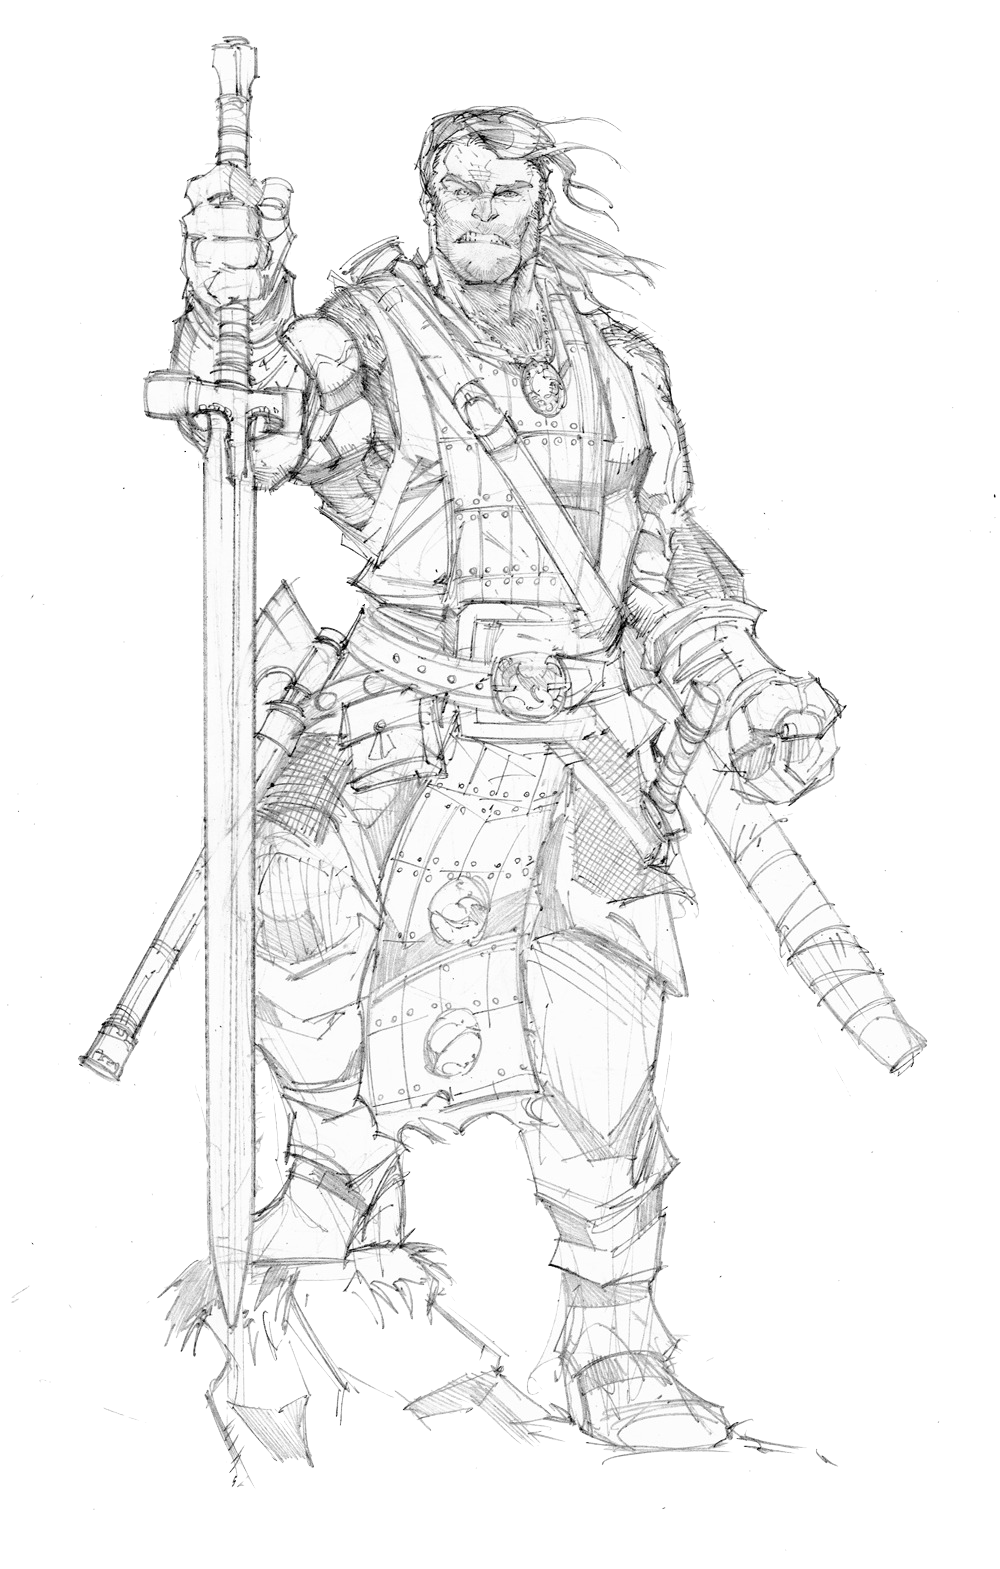
\includegraphics[width=\textwidth]{img/fighter.png}
 
AndronicusVII
\end{Figure}

\end{multicols*}    

\clearpage

\begin{table}[ht!]
\begin{small}
\rowcolors{2}{}{commentgreen}
\begin{center}
\begin{tabular}{ll}
\multicolumn{2}{l}{\parbox[l][0.6cm][c]{15cm}{\textbf{Fighter Maneuvers}}} 
\\
\hline 
\textbf{Name} & \parbox[l][0.6cm][c]{15cm}{\textbf{Description}}
\\ 
Goading Attack & \parbox[l][2.4cm][c]{15cm}{
When you hit a creature with a weapon attack, you can expend one stamina point to attempt to goad the target into attacking you. You add the stamina die to the attack's damage roll, and the target must make a Wisdom saving throw. On a failed save, the target has disadvantage on all attack rolls against targets other than you until the end of your next turn.
}
\\
Lunging Attack & \parbox[l][1.8cm][c]{15cm}{
When you make a melee \hl{two-handed} weapon attack on your turn, you can expend one stamina point to increase your reach for that attack by 5 feet. If you hit, you add the stamina die to the attack's damage roll.
}
\\
Maneuvering Attack & \parbox[l][2.4cm][c]{15cm}{
When you hit a creature with a \hl{reach} weapon attack, you can expend one stamina point to maneuver one of your comrades into a more advantageous position. You add the stamina die to the attack's damage roll, and you choose a friendly creature who can see or hear you. That creature can use its reaction to move up to half its speed without provoking opportunity attacks from the target of your attack.
}
\\
Menacing Attack & \parbox[l][2.1cm][c]{15cm}{
When you hit a creature with a weapon attack, you can expend one stamina point to attempt to frighten the target. You add the stamina die to the attack's damage roll, and the target must make a Wisdom saving throw. On a failed save, it is frightened of you until the end of your next turn.
}
\\
Pushing Attack & \parbox[l][2.2cm][c]{15cm}{
When you hit a creature with a \hl{bludgeoning} weapon attack, you can expend one stamina point to attempt to drive the target back. You add the stamina die to the attack's damage roll, and if the target is Large or smaller, it must make a Strength saving throw. On a failed save, you push the target up to 15 feet away from you.
}
\\
Trip Attack & \parbox[l][2cm][c]{15cm}{
When you hit a creature with a weapon attack, you can expend one stamina point to attempt to knock the target down. You add the stamina die to the attack's damage roll, and if the target is Large or smaller, it must make a Strength saving throw. On a failed save, you knock the target prone.
}
\\
Hold the Line & \parbox[l][2.8cm][c]{15cm}{
As a reaction when a hostile creature moves adjacent to an ally within 20 feet of you, you can spend one stamina point to immediately move up to your movement speed towards the creature. If you end your movement adjacent to the creature, make a Strength (Athletics) check contested by the target’s Strength (Athletics) or Dexterity (Acrobatics) check (the target chooses the ability to use). You add the stamina die to the roll. If you win the contest, you knock the target prone.
}
\\
Second wind & \parbox[l][1.6cm][c]{15cm}{
You have a limited well of stamina that you can draw on to protect yourself from harm. On your turn, you can spend one stamina point and use a bonus action to regain hit points equal to your stamina dice + your proficiency bonus.
}
\\
Shield block & \parbox[l][1.6cm][c]{15cm}{
When another creature hits you with a melee attack, you can use your reaction and expend one stamina point to increase your AC until the start of your next turn by the number you roll on your stamina die provided that you are holding a \hl{shield}.
}
\\
Precision Attack & \parbox[l][1.8cm][c]{15cm}{
When you make a weapon attack roll against a creature with a \hl{piercing} weapon, you can expend one stamina die to add it to the roll. You can use this maneuver before or after making the attack roll, but before any effects of the attack are applied.
}
\\
Riposte & \parbox[l][1.8cm][c]{15cm}{
When a creature misses you with a melee attack, you can use your reaction and expend one stamina point to make a melee weapon attack against the creature provided that you hold a \hl{sword}. If you hit, you add the stamina die to the attack's damage roll.
}
\\
\hline
\end{tabular}
\end{center}
\end{small}
\end{table}